% Proyecto final - Matemáticas Discretas (MAT 4021), Universidad del Norte
% Compilar con: pdfLaTeX + Biber (Overleaf lo hace automáticamente).
% Todo lo que dice \pendiente{...} (en rojo) son datos que el grupo debe completar.
\documentclass[11pt,a4paper]{article}

\usepackage[utf8]{inputenc}
\usepackage[T1]{fontenc}
\usepackage[spanish,es-tabla]{babel}
\usepackage[margin=2.5cm]{geometry}
\usepackage{amsmath,amssymb}
\usepackage{booktabs}
\usepackage{graphicx}
\usepackage{xcolor}
\usepackage{csquotes}
\usepackage{algorithm}
\usepackage{algpseudocode}
\usepackage[style=apa,backend=biber]{biblatex}
\DeclareLanguageMapping{spanish}{spanish-apa}
\addbibresource{referencias.bib}
\usepackage[hidelinks]{hyperref}

\newcommand{\pendiente}[1]{\textbf{\textcolor{red}{[#1]}}}
\renewcommand{\arraystretch}{1.15}

% Palabras clave del pseudocódigo en español
\algrenewcommand\algorithmicwhile{\textbf{mientras}}
\algrenewcommand\algorithmicdo{\textbf{hacer}}
\algrenewcommand\algorithmicfor{\textbf{para}}
\algrenewcommand\algorithmicif{\textbf{si}}
\algrenewcommand\algorithmicthen{\textbf{entonces}}
\algrenewcommand\algorithmicrequire{\textbf{Entrada:}}
\algrenewcommand\algorithmicensure{\textbf{Salida:}}
\algrenewcommand\algorithmicreturn{\textbf{devolver}}
\floatname{algorithm}{Algoritmo}

% Título provisional: cámbienlo si prefieren otro
\title{Asistente de ruta académica:\\ modelación del plan de estudios con grafos}
\author{Juan Ayala Díaz \and Bradley De La Hoz Guerrero \and Álvaro León Curvelo \and Alejandro Márquez Rincón\\[0.6em]
Matemáticas Discretas (MAT 4021)\\ Docente: MSc Iván Gómez\\ Universidad del Norte, Barranquilla}
\date{Noviembre de 2026}

\begin{document}
\maketitle

\begin{abstract}
Muchos estudiantes no saben qué materias se les bloquean cuando pierden o retiran una asignatura, cuáles pueden matricular ni cómo se acumulan sus créditos y su promedio. Este trabajo modela el plan de estudios de Ingeniería de Sistemas y Computación de la Universidad del Norte como un grafo dirigido acíclico, cuyos vértices son materias con créditos y cuyas aristas son prerrequisitos y correquisitos. Sobre ese modelo se implementó un programa en Python que, a partir del historial del estudiante, responde qué materias puede matricular, qué se bloquea si pierde o retira una materia, cuántos semestres le faltan como mínimo y cómo cambia su promedio. El programa se validó con un caso real: reproduce exactamente el promedio general acumulado (3.70) que reporta la aplicación de la universidad. Se aplican además el álgebra booleana (la regla de matrícula como función lógica, verificada por equivalencia), medidas de centralidad (importancia de cada materia) y un perceptrón. En una encuesta a 43 estudiantes, 65 \% no sabe con exactitud cuántos créditos ha aprobado y 42 \% no sabe con seguridad qué materias se le bloquean. \pendiente{agregar el resultado de la medición antes/después}

\medskip
\noindent\textbf{Palabras clave:} grafos dirigidos acíclicos, prerrequisitos, álgebra booleana, centralidad, perceptrón, plan de estudios, Python.

\medskip\noindent\textbf{Repositorio:} \url{https://github.com/AmilJoJoTard/Asistente-de-ruta-academica} \pendiente{reemplazar por el enlace real}
\end{abstract}

\section{Introducción}

\subsection{El problema}
En la universidad, cada materia tiene prerrequisitos y un número de créditos, y esas reglas se encadenan: perder una materia puede impedir ver otras varios semestres después. Un estudiante que pierde o retira una materia con frecuencia no sabe cuáles materias se le bloquean, cuáles puede matricular ese semestre ni cuánto afecta eso a su ruta. Además, pocos consultan el plan de estudios completo, y calcular los créditos acumulados o el efecto de una nota sobre el promedio resulta difícil a mano.

\subsection{Por qué es un problema de impacto}
La Tabla~\ref{tab:impacto} resume las cuatro condiciones de un problema de impacto.

\begin{table}[htbp]
\centering
\caption{Condiciones de impacto del problema}
\label{tab:impacto}
\begin{tabular}{p{3.3cm}p{11.2cm}}
\toprule
Condición & Respuesta del proyecto \\
\midrule
Afecta a alguien & Estudiantes de pregrado de la Universidad del Norte. La coordinación del programa no dispone de la cifra de estudiantes activos, así que el alcance se documenta con una encuesta (43 respuestas de 17 programas). \\
Hay evidencia & Encuesta propia (Tabla~\ref{tab:encuesta}): 65 \% no sabe con exactitud cuántos créditos ha aprobado y 42 \% no sabe con seguridad qué materias se le bloquean si pierde o retira una. \\
Se puede mejorar & Se puede medir el tiempo y los errores al planear la ruta a mano frente a usar el programa. En la encuesta, 65 \% tarda más de 30 minutos en planear su matrícula. \pendiente{medición con el programa (después)} \\
Se puede modelar & Grafos dirigidos acíclicos: prerrequisitos, dependencias en cadena y caminos más largos. \\
\bottomrule
\end{tabular}
\end{table}

\subsection{Evidencia: encuesta a estudiantes}
Se aplicó una encuesta anónima y voluntaria con Google Forms, difundida por grupos de estudiantes. Respondieron 43 personas de 17 programas (16 de Ingeniería de Sistemas); 36 de ellas (84 \%) cursan segundo o tercer semestre. Es una muestra por conveniencia: no representa a toda la universidad y sirve como evidencia de que el problema existe, no para estimar su tamaño exacto. La Tabla~\ref{tab:encuesta} resume los resultados.

\begin{table}[htbp]
\centering
\caption{Resultados de la encuesta ($n=43$)}
\label{tab:encuesta}
\begin{tabular}{p{9.6cm}rr}
\toprule
Pregunta & Personas & \% \\
\midrule
No sabe con exactitud cuántos créditos ha aprobado & 28 & 65 \\
Solo ha revisado una parte del pensum de su carrera & 16 & 37 \\
No sabe con seguridad qué materias se le bloquean si pierde o retira una & 18 & 42 \\
No puede calcular con seguridad cuánto bajaría su promedio si pierde una materia & 20 & 47 \\
Descubrió tarde (o casi) que no podía ver una materia por un prerrequisito & 7 & 16 \\
Ha dudado entre retirar o perder una materia sin saber las consecuencias & 16 & 37 \\
Tarda más de 30 minutos en planear su matrícula & 28 & 65 \\
Califica con 4 o 5 (de 5) la utilidad de una herramienta como la propuesta & 37 & 86 \\
\bottomrule
\end{tabular}
\end{table}

Entre las 12 personas que han perdido o retirado alguna materia, 8 (67 \%) dudaron entre retirar o perder, frente a 8 de 31 (26 \%) entre quienes no han perdido ni retirado. La función que más usarían es la simulación del promedio (35 \%), seguida de ver qué se bloquea (26 \%), qué pueden matricular el próximo semestre (21 \%) y sus créditos y avance (19 \%). En los comentarios abiertos hubo peticiones de priorizar las materias por importancia o dificultad, que se aborda con el puntaje de importancia (Sección~\ref{sec:importancia}), y de simular horarios, que queda como trabajo futuro.

\subsection{Objetivos}
\textbf{Objetivo general.} Modelar el plan de estudios de Ingeniería de Sistemas y Computación como un grafo y construir un programa que oriente a los estudiantes sobre su ruta académica.

\textbf{Objetivos específicos.}
\begin{itemize}
  \item Representar materias, créditos, prerrequisitos y correquisitos como un grafo dirigido.
  \item Determinar qué materias puede matricular un estudiante y cuáles se bloquean si pierde o retira una.
  \item Calcular créditos, semestres mínimos restantes y promedio ponderado.
  \item Aplicar álgebra booleana, medidas de centralidad y un perceptrón para explicar y apoyar las decisiones del estudiante.
  \item Validar el programa con un caso de resultado conocido.
\end{itemize}

\section{Modelación con la teoría del curso}

\subsection{El plan de estudios como grafo}
Sea $G=(V,E)$ un grafo dirigido donde $V$ es el conjunto de materias y $c:V\to\mathbb{N}$ asigna a cada materia sus créditos. El conjunto de aristas se divide en $E=E_p\cup E_c$: una arista $(u,v)\in E_p$ indica que $u$ es prerrequisito de $v$, y una arista $(u,v)\in E_c$, que $u$ es correquisito de $v$. El subgrafo de prerrequisitos $G_p=(V,E_p)$ debe ser acíclico: si tuviera un ciclo, ninguna de las materias del ciclo podría cursarse \parencite{rosen2019}. El programa verifica esta propiedad al cargar el plan.

El plan de Sistemas modelado tiene 62 vértices (32 obligatorias, 18 electivas, 8 niveles de idiomas, 2 exámenes comprehensivos y 2 seminarios), 40 aristas (39 de prerrequisito y 1 de correquisito) y 155 créditos en total. La Figura~\ref{fig:grafo} muestra las materias obligatorias.

\begin{figure}[htbp]
\centering
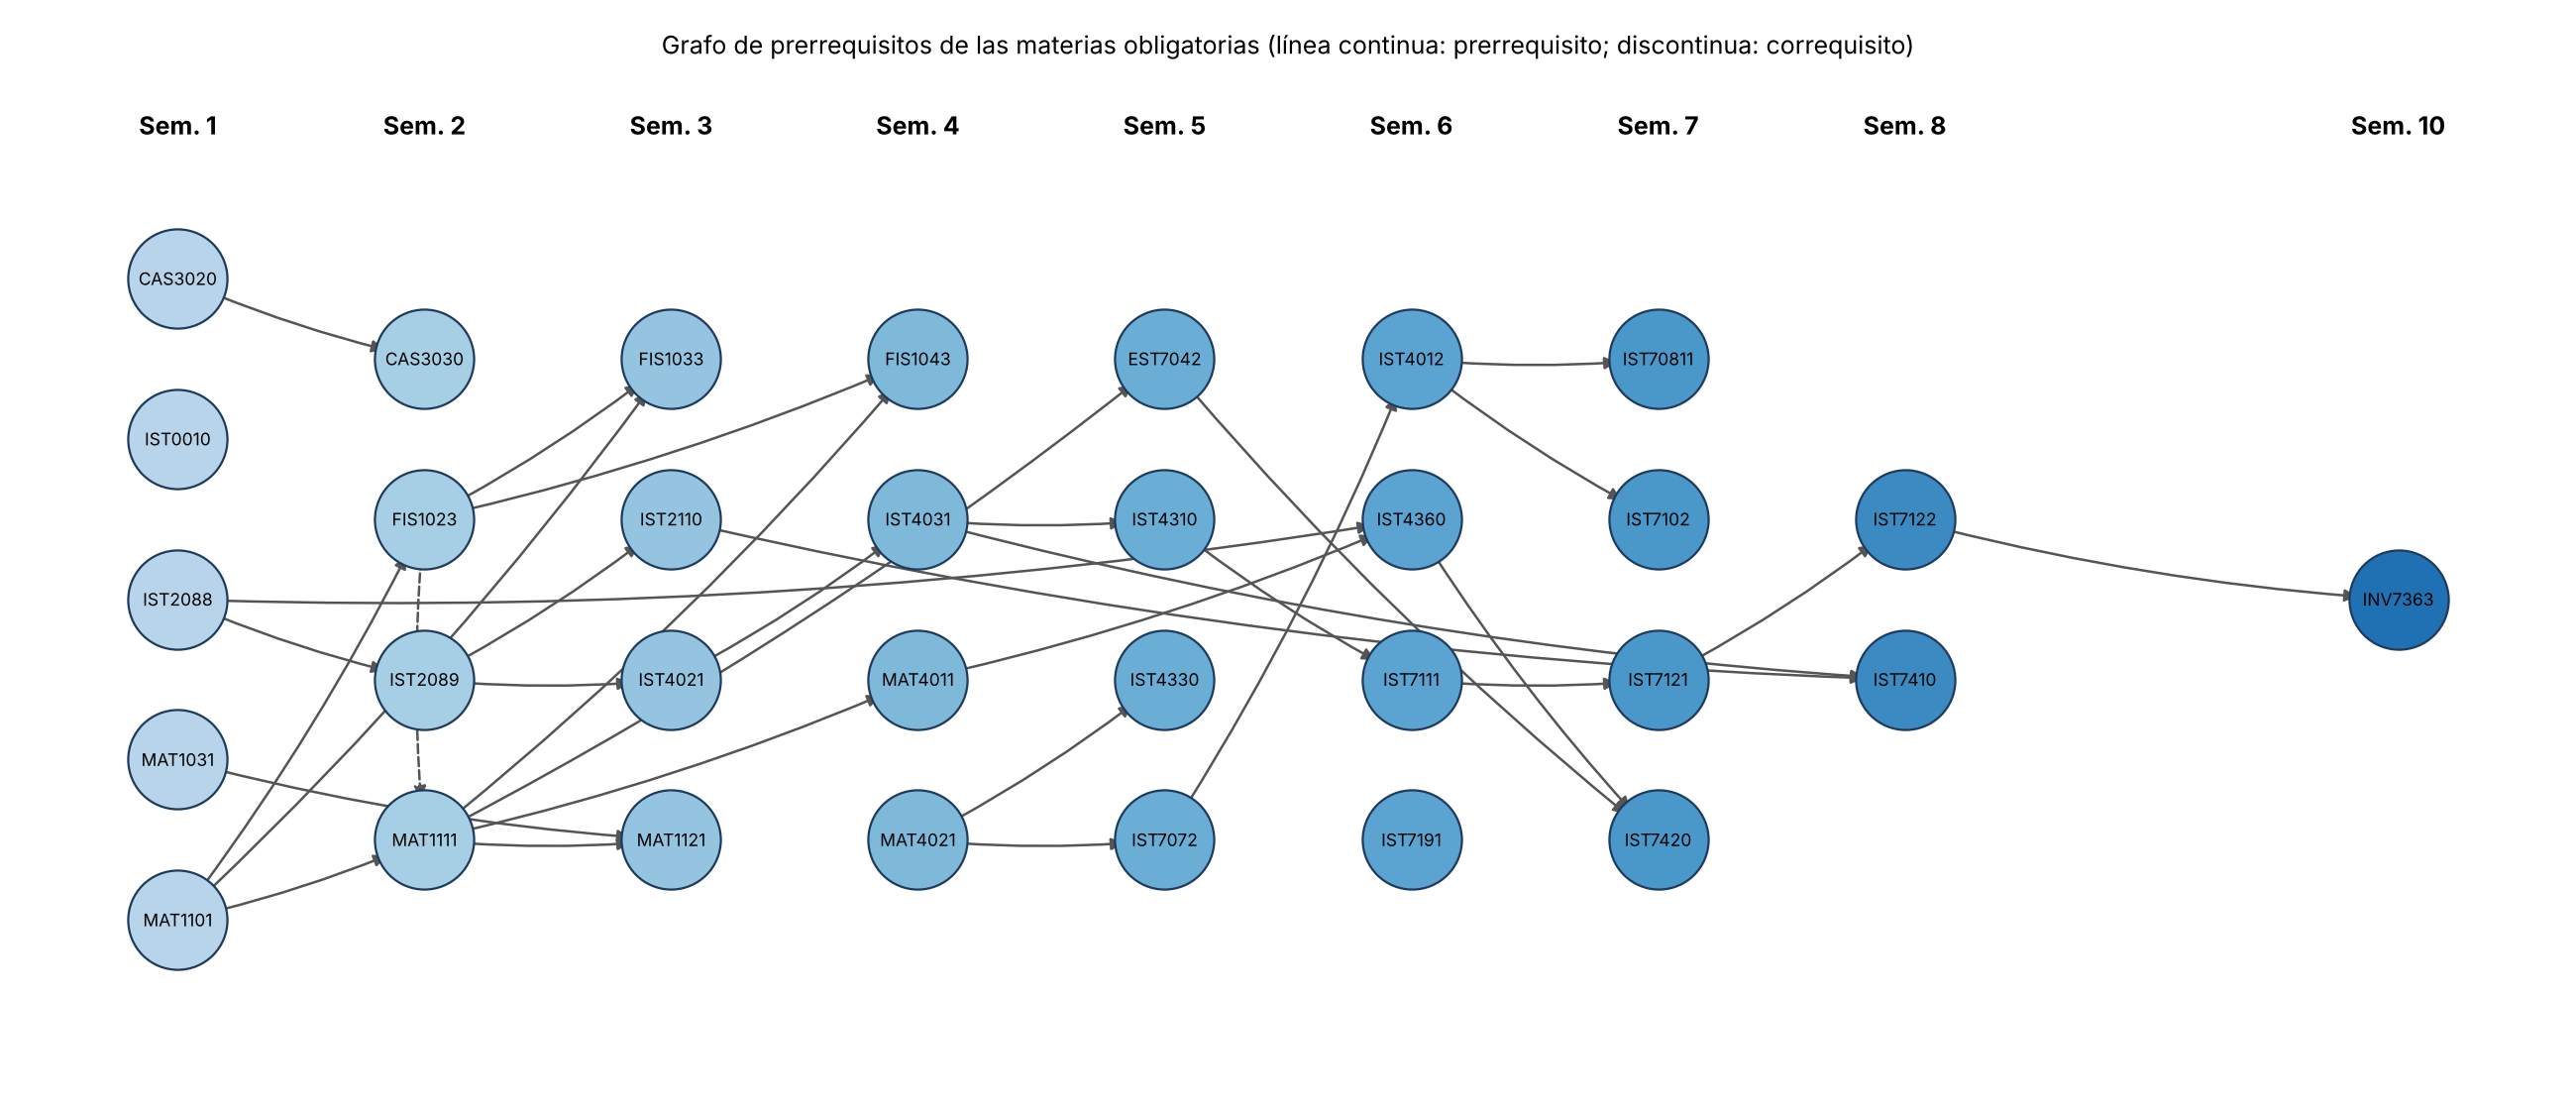
\includegraphics[width=\textwidth]{figuras/grafo_pensum.png}
\caption{Grafo de prerrequisitos de las materias obligatorias de Ingeniería de Sistemas y Computación.}
\label{fig:grafo}
\end{figure}

\subsection{Estados y materias disponibles}
El historial del estudiante asigna a cada materia un estado $\sigma(v)$: aprobada, perdida, retirada, cursando o sin cursar. Una materia es \emph{pendiente} si $\sigma(v)\notin\{\text{aprobada},\text{cursando}\}$. El conjunto de materias que puede matricular es
\begin{multline*}
D(\sigma)=\Big\{v\ \text{pendiente}:\ \forall (u,v)\in E_p,\ \sigma(u)=\text{aprobada}\ \ \text{y}\\
\forall (u,v)\in E_c,\ \sigma(u)\in\{\text{aprobada},\text{cursando}\}\Big\}.
\end{multline*}

\subsection{Bloqueos en cadena}
Si el estudiante pierde o retira una materia $x$, las materias que dependen de ella directa o indirectamente son los descendientes de $x$ en $G_p$:
\[
B(x)=\{v\in \operatorname{Desc}_{G_p}(x):\ \sigma(v)\neq\text{aprobada}\}.
\]
Cuanto mayor es $|B(x)|$, más crítica es la materia $x$.

\subsection{Créditos y semestres mínimos}
Los créditos aprobados son $\sum_{v:\,\sigma(v)=\text{aprobada}} c(v)$. Para estimar cuántos semestres faltan se combinan dos cotas inferiores: la longitud $L$ del camino más largo en el subgrafo de $G_p$ inducido por las materias pendientes (que obliga a cursarlas en semestres distintos, un vértice por semestre como mínimo) y la cota por créditos $\lceil C_{pend}/C_{max}\rceil$, donde $C_{pend}$ son los créditos pendientes y $C_{max}$ el máximo permitido por semestre:
\[
S_{min}=\max\big(L+1,\ \lceil C_{pend}/C_{max}\rceil\big).
\]
En un DAG, el camino más largo se calcula en tiempo lineal con un recorrido en orden topológico \parencite{cormen2022}.

\subsection{Promedio ponderado}
Sea $A$ el conjunto de intentos con nota que cuentan para el promedio, es decir, los aprobados y los perdidos. Cada intento $i$ tiene nota $n_i\in[0,5]$ y créditos $c_i$. El promedio general acumulado es
\[
\mathrm{PGA}=\frac{\sum_{i\in A} n_i\,c_i}{\sum_{i\in A} c_i}.
\]
Las materias retiradas y las que se están cursando no entran en $A$. Retirar una materia no cambia el promedio, mientras que perderla sí. Con los datos del caso real se comprobó que cada intento cuenta, incluso si la materia se repite después.

\subsection{Reglas de la universidad incorporadas}
\begin{itemize}
  \item \textbf{Electivas:} cada código electivo representa un cupo de créditos que admite muchas materias reales.
  \item \textbf{Idiomas:} no son prerrequisitos entre sí, porque un examen de ubicación permite empezar en cualquier nivel. Al aprobar un nivel, los inferiores quedan cubiertos y solo se ofrece el siguiente; el examen de ubicación puede repetirse con costo adicional. Los idiomas se pagan aparte de la matrícula y tienen 0 créditos.
  \item \textbf{Carga y retiros:} según el Reglamento de Estudiantes \parencite{uninorte2012}, en Ingenierías la carga normal es de 7 a 17 créditos por semestre (art.~68), las asignaturas se pueden retirar hasta la semana 14 y quedan como no cursadas (arts.~57 y 58), y una materia se aprueba con 3.0 (art.~98), con 1.5 como nota definitiva mínima (art.~102). Según la coordinación del programa, tampoco se puede retirar una materia si el estudiante queda con menos de 7 créditos.
  \item \textbf{Matrícula:} solo se pueden matricular materias de tres semestres consecutivos del plan, y primero se matriculan las perdidas y luego las más atrasadas (art.~51). Por eso el programa calcula una \emph{ventana} de semestres que empieza en la materia pendiente más atrasada. La universidad no abre todas las materias cada semestre; adelantar una requiere hablar con la coordinación del programa.
  \item \textbf{Estado académico:} el promedio mínimo exigido es 3.25, y el estado de estudiante distinguido exige 3.95 con al menos 16 créditos (arts.~124 a 130). Según la coordinación, quien baja del mínimo entra en período de prueba: se observa su desempeño el semestre siguiente, se le cita si empeora y, en último caso, puede no poder matricularse. El programa muestra el estado estimado y cómo cambiaría si el estudiante pierde una materia.
\end{itemize}

\subsection{Álgebra booleana: la regla de matrícula}
\label{sec:booleano}
Para cada materia $x$ se definen dos variables booleanas: $A_x$ (``$x$ está aprobada'') y $C_x$ (``$x$ se está cursando''). La combinación $A_x=C_x=1$ es imposible, así que se trata como un \emph{don't care}. La regla de matrícula es la función booleana
\[
\mathrm{Disp}(v)=\overline{A_v}\cdot\overline{C_v}\cdot\prod_{u\in P(v)}A_u\cdot\prod_{w\in K(v)}(A_w+C_w),
\]
donde $P(v)$ son los prerrequisitos de $v$ y $K(v)$ sus correquisitos. Para Cálculo II (prerrequisito: Cálculo I; correquisito: Física Mecánica), la parte de requisitos es $R=A_{C1}\,(A_{F}+C_{F})$, con forma canónica $\Sigma m(5,6)+d(3,7)$. Al simplificarla con Quine--McCluskey, que equivale a agrupar en un mapa de Karnaugh aprovechando los \emph{don't cares}, queda $R=A_{C1}A_{F}+A_{C1}C_{F}$. Por De Morgan, $\overline{R}=\overline{A_{C1}}+\overline{A_{F}}\,\overline{C_{F}}$, y cada término de $\overline{R}$ es una razón por la que el estudiante no puede matricular la materia. Una materia sin requisitos tiene $R=1$, que es una tautología. Con esto el programa responde Sí o No y explica por qué.

\subsection{Importancia de cada materia}
\label{sec:importancia}
La red de prerrequisitos es dirigida ($u\to v$ si $u$ es prerrequisito de $v$) y tiene varias componentes conexas, por lo que la cercanía se calcula con la variante armónica y no con la suma de distancias. Para cada materia se calculan el grado de salida (materias que se abren directamente al aprobarla), el alcance (materias que dependen de ella directa o indirectamente) y la intermediación (fracción de los caminos más cortos entre otras materias que pasan por ella). Con ellas y los créditos se define un puntaje de importancia en $[0,1]$:
\[
I(v)=0.2\,\hat c(v)+0.5\,\hat b(v)+0.3\,\hat p(v),
\]
donde $\hat c$, $\hat b$ y $\hat p$ son los créditos, el alcance y la intermediación divididos entre su valor máximo. Los pesos son una decisión de modelación: se privilegia el bloqueo porque es lo que le cuesta al estudiante perder la materia. Si se contara con la dificultad percibida (de 1 a 5), podría añadirse como cuarto componente.

\subsection{Perceptrón: ¿aprobará la materia?}
\label{sec:perceptron}
Un perceptrón con entradas $x_1,\dots,x_n$ calcula $z=\sum_i w_i x_i+b$ y predice $\hat y=\varphi(z)$, con $\varphi$ la función escalón ($1$ si $z\ge 0$ y $0$ en otro caso). Se entrena con la regla $w_i\leftarrow w_i+\gamma\,(y-\hat y)\,x_i$ y $b\leftarrow b+\gamma\,(y-\hat y)$, con tasa de aprendizaje $\gamma=0.05$, pesos iniciales cero y sesgo inicial $0.122$. Se aplica a una clasificación binaria: dada la nota en una materia previa (dividida entre 5), predecir si la nota en la siguiente será al menos 3.0. La implementación reproduce el entrenamiento del AND visto en clase: tras tres pasos, $w=(-0.05,-0.05)$ y $b=-0.028$, y con más épocas aprende la función completa. No se recolectaron parejas de notas de estudiantes reales, así que el perceptrón no se evaluó con datos reales: el módulo queda como demostración del método y se plantea como trabajo futuro entrenarlo con notas recolectadas de forma anónima y evaluarlo contra el modelo trivial de predecir siempre la clase más común.

\section{Solución: algoritmos y datos}

\subsection{Datos}
El plan de estudios se transcribió del plan publicado por la universidad (programa con código SNIES 103821) a tres archivos: materias con sus créditos y semestre, prerrequisitos y reglas de la carrera. Un integrante confirmó cada prerrequisito. El historial del estudiante se lee de un archivo CSV con el código de la materia, el periodo, el estado y, opcionalmente, la nota. \pendiente{citar la fuente oficial del plan de estudios con fecha de consulta}

\subsection{Algoritmos}
El Algoritmo~\ref{alg:bloqueadas} calcula las materias bloqueadas con una búsqueda en anchura sobre $G_p$, y el Algoritmo~\ref{alg:disponibles} calcula las materias disponibles.

\begin{algorithm}[htbp]
\caption{Materias bloqueadas por una materia $x$}
\label{alg:bloqueadas}
\begin{algorithmic}[1]
\Require grafo de prerrequisitos $G_p=(V,E_p)$, materia $x$, estados $\sigma$
\Ensure conjunto $B$ de materias no aprobadas que dependen de $x$
\State $B\gets\emptyset$;\quad $Q\gets[x]$
\While{$Q$ no esté vacía}
  \State $u\gets$ sacar el primer elemento de $Q$
  \For{cada arista $(u,v)\in E_p$}
    \If{$v\notin B$}
      \State agregar $v$ a $B$ y a $Q$
    \EndIf
  \EndFor
\EndWhile
\State \Return $\{v\in B:\ \sigma(v)\neq\text{aprobada}\}$
\end{algorithmic}
\end{algorithm}

\begin{algorithm}[htbp]
\caption{Materias disponibles}
\label{alg:disponibles}
\begin{algorithmic}[1]
\Require grafo $G=(V,E_p\cup E_c)$, estados $\sigma$
\Ensure conjunto $D$ de materias que se pueden matricular
\State $D\gets\emptyset$
\For{cada materia pendiente $v\in V$}
  \If{todo prerrequisito de $v$ está aprobado \textbf{y} todo correquisito está aprobado o cursándose}
    \State agregar $v$ a $D$
  \EndIf
\EndFor
\State \Return $D$
\end{algorithmic}
\end{algorithm}

Ambos algoritmos recorren cada vértice y cada arista una vez, por lo que su costo es $O(|V|+|E|)$. Para el plan de Sistemas ($|V|=62$, $|E|=40$) la respuesta es inmediata. Para el siguiente semestre se supone que el estudiante aprueba lo que cursa y se vuelve a calcular $D$; la carga sugerida prioriza las materias con mayor $|B(x)|$ sin superar el máximo de créditos y completa con electivas hasta el mínimo.

\subsection{Implementación}
El programa está escrito en Python y usa la biblioteca NetworkX para los grafos \parencite{hagberg2008}. Se organiza en módulos de carga de datos, construcción y validación del grafo, consultas, promedio, álgebra booleana, importancia de materias, perceptrón y una interfaz de consola con un menú de preguntas. Incluye 72 pruebas automáticas con \texttt{pytest} y un archivo README con las instrucciones para ejecutarlo. El código fuente, los datos y la documentación para reproducir los resultados están en el repositorio del proyecto: \url{https://github.com/AmilJoJoTard/Asistente-de-ruta-academica} \pendiente{enlace real}.

\section{Resultados e interpretación}

\subsection{Validación con un caso real}
Para validar el cálculo del promedio se usó el historial de un estudiante de Sistemas con dos semestres cerrados (Tabla~\ref{tab:validacion}). La aplicación de la universidad reporta un PGA de 3.70 (la propia aplicación aclara que sus notas son una guía y no oficiales).

\begin{table}[htbp]
\centering
\caption{Intentos que cuentan para el promedio en el caso de validación}
\label{tab:validacion}
\begin{tabular}{lrrlr}
\toprule
Materia & Créditos & Nota & Estado & Nota $\times$ créditos \\
\midrule
IST0010 & 1 & 4.8 & aprobada & 4.8 \\
IST2088 & 3 & 2.5 & perdida & 7.5 \\
MAT1031 & 3 & 3.4 & aprobada & 10.2 \\
CAS3020 & 3 & 3.9 & aprobada & 11.7 \\
IGL1030 & 0 & 4.0 & aprobada & 0.0 \\
MAT1101 & 5 & 3.0 & aprobada & 15.0 \\
IST2088 & 3 & 3.8 & aprobada & 11.4 \\
CAS3030 & 3 & 4.5 & aprobada & 13.5 \\
ELG1140 & 3 & 4.9 & aprobada & 14.7 \\
ELG1130 & 3 & 3.7 & aprobada & 11.1 \\
\midrule
Total & 27 & & & 99.9 \\
\bottomrule
\end{tabular}
\end{table}

Una materia retirada (Cálculo I en el primer semestre) no entra al cálculo. El programa obtiene $99.9/27=3.70$, igual al valor de la aplicación. Si solo contara el último intento de cada materia, el resultado sería 3.85, que no coincide; esto confirma que la universidad cuenta todos los intentos.

\subsection{Simulaciones}
Con el mismo historial, el programa estima cuánto bajaría el promedio si el estudiante perdiera Algoritmia y Programación II (3 créditos), que cursa actualmente (Tabla~\ref{tab:simulacion}). La nota definitiva mínima es 1.5 (art.~102). En todos los casos el estudiante seguiría por encima del mínimo de 3.25 y en estado normal. Si retira la materia, el promedio se mantiene en 3.70.

\begin{table}[htbp]
\centering
\caption{Promedio si se pierde una materia de 3 créditos}
\label{tab:simulacion}
\begin{tabular}{rrr}
\toprule
Nota obtenida & Nuevo promedio & Cambio \\
\midrule
1.5 & 3.48 & $-0.22$ \\
2.0 & 3.53 & $-0.17$ \\
2.5 & 3.58 & $-0.12$ \\
2.9 & 3.62 & $-0.08$ \\
\bottomrule
\end{tabular}
\end{table}

En cuanto a los bloqueos, no aprobar Algoritmia y Programación I bloquea 12 materias en cadena, entre ellas Proyecto Final, y retirar Cálculo II bloquea 7 (Cálculo III, Ecuaciones Diferenciales, Física Electricidad, Análisis de Datos I, Soluciones Computacionales, Optimización y el Examen Comprehensivo I). Desde cero, el camino más largo de prerrequisitos obliga a cursar al menos 9 semestres, y el tope de 17 créditos por semestre obliga a al menos 10, que es la duración del plan. Para el historial del caso, la ventana de matrícula abarca los semestres 2 a 4 del plan, de modo que el próximo semestre el programa sugiere 14 créditos: Cálculo II, Física Calor-Ondas, Programación Orientada a Objetos y Estructura de Datos I.

\subsection{Verificación de la lógica booleana}
Se comprobó que la expresión booleana de cada una de las 62 materias coincide con la implementación basada en el grafo en las 17\,750 combinaciones de estados de las materias involucradas, sin ninguna diferencia. Es una prueba exhaustiva de equivalencia lógica, equivalente a comparar ambas tablas de verdad.

\subsection{Materias más críticas}
La Tabla~\ref{tab:importancia} muestra las cinco materias con mayor puntaje de importancia. Dominan las de la cadena de programación: Estructura de Datos II y Algoritmia y Programación II combinan un bloqueo alto con un papel de puente, mientras que Algoritmia y Programación I es la que más materias bloquea (12) pero no es puente, porque no hay caminos que pasen por ella.

\begin{table}[htbp]
\centering
\caption{Materias más críticas del plan de Sistemas}
\label{tab:importancia}
\begin{tabular}{lrrrr}
\toprule
Materia & Créditos & Bloquea & Puente & Puntaje \\
\midrule
Estructura de Datos II & 3 & 6 & 0.014 & 0.67 \\
Algoritmia y Programación II & 3 & 9 & 0.008 & 0.66 \\
Estructura de Datos I & 3 & 7 & 0.011 & 0.64 \\
Algoritmia y Programación I & 3 & 12 & 0.000 & 0.62 \\
Cálculo I & 5 & 10 & 0.000 & 0.62 \\
\bottomrule
\end{tabular}
\end{table}

\subsection{Interpretación}
Las materias con más descendientes, como Algoritmia y Programación I, son las más críticas: perder una de ellas retrasa muchas otras. Perder una materia afecta al promedio en proporción a sus créditos y a la distancia entre la nota obtenida y el promedio actual, mientras que retirarla lo deja intacto. El programa pone esos efectos a la vista antes de que el estudiante decida.

\pendiente{agregar aquí los resultados de la medición antes/después con estudiantes}

\section{Conclusiones y limitaciones}
\subsection{Conclusiones}
\begin{itemize}
  \item El plan de estudios se modela de forma natural como un DAG, y consultas que el estudiante hace a mano (disponibles, bloqueos, semestres mínimos) se resuelven con recorridos de grafos en tiempo lineal.
  \item El programa reproduce el promedio oficial de un caso real, lo que respalda la validez del modelo.
  \item La regla de matrícula, escrita como función booleana, equivale exactamente a la implementación del grafo, y sus términos explican al estudiante por qué una materia no está disponible.
  \item Las medidas de centralidad identifican qué materias son más críticas, como insumo para decidir qué retirar o priorizar.
  \item Como las reglas de cada carrera son datos y no código, el modelo puede extenderse a otros programas de la universidad.
\end{itemize}

\subsection{Limitaciones}
\begin{itemize}
  \item Solo se modeló Ingeniería de Sistemas y Computación.
  \item La encuesta es una muestra por conveniencia (43 personas, 84 \% de segundo y tercer semestre) y no se dispone de la cifra oficial de estudiantes activos.
  \item No se contó con datos de notas para evaluar el perceptrón con estudiantes reales, por lo que ese módulo es solo una demostración del método.
  \item El programa no conoce qué materias abre realmente la universidad cada semestre: muestra lo que el reglamento permite matricular, y adelantar una materia requiere hablar con la coordinación del programa. Además, según la coordinación, el nivel de idiomas puede limitar las materias que se ofrecen, regla que el programa todavía no modela.
  \item Los idiomas se modelan de forma simplificada (nivelación y orden), sin los detalles del examen de ubicación.
  \item Las notas de la aplicación de la universidad son una guía no oficial, y el caso de validación es uno solo.
  \item La herramienta orienta, pero no reemplaza al sistema de registro ni a la asesoría académica.
\end{itemize}

\printbibliography[title=Referencias]

\end{document}
